\minitoc  % Affiche la table des matières pour ce chapitre

% ==================================================================================================================================
% Introduction 

Dans ce chapitre, nous allons essayer d'étudier les propriétés de fonctions en les assimilant à leur classe d'équivalence 
pour l'égalité presque partout. Nous allons d'abord commencer par montrer que c'est possible. Ensuite nous verrons quelques propriétés
des espaces de ces "classes d'équivalences" et nous finirons par étudier le produit de convolution dans ces espaces. 

% ==================================================================================================================================
% Espaces Lp

\section{Espaces $L^p$}

\subsection{Intégration et égalité presque partout}

Soit $(X,\mathcal{B},\mu)$ un espace mesuré et $\mathcal{M}(X) = \{f : X \rightarrow \C\}$ l'ensemble des fonctions mesurables 
de X. On sait que $ f \sim_{\text{p.p}} g \; \Longleftrightarrow \; f = g \text{ p.p } \Longleftrightarrow \mu (\{ x \in X, \; f(x) \not = g(x) \}) = 0 $. 

Donc l'égalité presque partout est une relation d'équivalence telle que :
    \[ M(X) := \mathcal{M}(X) / \sim_{\text{p.p}} \] 

On différenciera bien les M dits "droits" et les $\mathcal{M}$ dit "courbes". 
Les premiers représentent classes d'équivalences des fonction de $\mathcal{M}$ pour la relation d'égalité presque partout. 

\begin{remark}
    Soit $f \in M(X)$ et x$ \in X$, $f(x)$ n'a aucun sens cet $f$ n'est pas une fonction mais une classe d'équivalence de fonctions. 
\end{remark}

\begin{example}[Fonctions de même classe]
    Plaçons nous dans $(\R,\mathcal{B}_\R,\lambda)$ avec $f = 0$ et $g = 1_{\{0\}}$, on remarquera que $f = g$ p.p. 
    Donc $f$ et $g$ sont de même classe. 
\end{example}

\begin{definition}[Intégrale d'une classe]
    Soit $f \in \overline{\mathcal{M}_+}(X)$ (ici une classe), l'intégrale de $f$ est définie par :
        \[ \int f \;d \mu := \int f_1 \; d \mu \] 
    Où $f_1$ est une fonction de la classe $f$. 
\end{definition}

\begin{remark}
    On s'appuie sur la propriété suivante :
    \begin{quote}
        Soit $M(X)$ une classe d'équivalence de $\mathcal{M}(X)$, alors $ \forall f_1,f_2 \in M(X)$, on a :
            \[ \int_X f_1 \; d \mu = \int_X f_2 \; d \mu \] 
        i.e l'intégrale de la classe ne dépend pas du représentant de la classe. 
    \end{quote}
\end{remark}


\begin{definition}[Espace $L^p$]
    On définit de même les ensembles $L^p$, les classes d'équivalences des fonctions intégrables pour la relation d'égalité 
    presque partout : 
    \begin{itemize}
        \item si $p=1$, on a : $ L^1(X) = \{ f \in M(X), \; \int_x |f| \; d \mu < \infty \} $
        \item si $p < \infty$, on a : $L^p(X) = \{ f \in M(X), \; \int_x |f|^p \; d \mu < \infty \}$
        \item si $p = \infty$, on a : $L^\infty(X) = \{ f \in M(X), \; \exists C \in R_+^*, \; |f| \leq C \}$
    \end{itemize}
    où $f$ est la classe de $f_1$ pour tout fonction $f_1$ de la classe $f$.
\end{definition}

\begin{theorem}[Extension]
    Tous les théorèmes et définitions du cours d'intégration sont applicables aux classes de fonctions. 
\end{theorem}

$L^\infty$ est l'ensemble des classes de fonctions "grosso-modo" bornées. 


\subsection{Espace $L^p$}

\begin{definition}[Normes $L^p$]
    Soient $f \in M(X)$ et $p \in [1;\infty[$ on définit les normes suivantes :
    \[ 
        \|f\|_p = \Big( \int_X |f|^p \; d \mu \Big)^{\frac{1}{p}} \qquad 
        \|f\|_\infty  = \inf \Bigl\{ C \in \overline{R_+}, \; |f| \leq C \text{ p.p} \Bigr\}
    \]
\end{definition}

\begin{prop}
    Soit $f \in M(X)$ et $p \in [1,\infty]$ on a :
        \[ f \in L^p(X) \; \Longleftrightarrow \; \|f\|_p < \infty \]
\end{prop}

\begin{theorem}[Inégalité de Holder]
    Soient $p,q,r \in [1,\infty]$ tels que :
        \[ \boxed{ \frac{1}{p} + \frac{1}{q} = \frac{1}{r} \; \Longrightarrow \; \forall f,g \in M(X), \; \|fg\|_r \leq \|f\|_p \times \|g\|_q } \] 
\end{theorem}

\begin{theorem}[Inégalité de Young]
    Pour tous $p,q,r \in [1,\infty]$, on a :
        \[ \forall a,b \in \R_+, \quad \frac{a^p}{p} + \frac{b^p}{q} \] 
\end{theorem}

\begin{remark} 
    Quelques cas particuliers de l'inégalité de Holder :
    
    \begin{itemize}
        \item $ \|fg\|_\infty \leq \| f \|_\infty \times \|g\|_\infty $
        \item $ \|fg\|_p \leq \|f\|_\infty \times \|g\|_p $
        \item $ \|fg\|_1 \leq \|f\|_2 \times \|g\|_2 $
    \end{itemize}
\end{remark}

\begin{remark} Conséquence de l'inégalité de Holder :
    Si $ \forall f,g \in M(X), \; \|fg\|_r \leq \|f\|_p \times \|g\|_q$ alors on peut dire que :
        \[ L^p(X) L^q(X) \subseteq L^r(X) \] 
\end{remark}

\begin{theorem}[Structure des espaces $L^p$]
    L'espace $(L^p(X), \|.\|_P)$ est un espace vetoriel normé, complet
    (i.e toutes les suites de Cauchy convergent).
\end{theorem}

\begin{remark}[Rappel suites de Cauchy]
    Soit $(u_n) \in X^\N$ une suite de X. On dit que c'est une suite de Cauchy si :
        \[ \forall \varepsilon > 0, \exists n_0 \in \N, \forall n,p \geq n_0, \quad \| u_n - u_p\| < \varepsilon \] 
    i.e \emph{à partir d'une certain rang tous les termes de la suite se rapprochent autant qu'on veut.}
    
    On remarquera d'une suite convergente est "de Cauchy" mais la réciproques n'est pas tout le temps vraie. 
\end{remark}

\begin{theorem}[Structure de $L^2$]
    $L^2$ est un \textbf{espace préhilbertien} complet muni du produit scalaire suivant :
    \[ \text{où} \quad \langle .,. \rangle : 
        \begin{cases}
            L^2 \times L^2 \longrightarrow \C \\ 
            (f,g) \longmapsto \int f \overline{g} \; d \mu 
        \end{cases}
    \]
    C'est un produit scalaire hermitien, de plus, bien défini car le produit de deux fonctions $L^2$ est $L^1$. 
\end{theorem}

\begin{remark}[Espaces de Banach, espaces de Hilbert] Posons quelques mots de vocabulaire sur les espaces définis :
    \begin{itemize}
        \item Un espace vectoriel muni d'un produit scalaire appelé \textbf{espace préhilbertien}.
        \item Un espace vectoriel normé, complet est appelé \textbf{espace de Banach}. 
        \item Un espace préhilbertien complet est appelé \textbf{espace de Hilbert}.
    \end{itemize}
\end{remark}

\begin{remark}[Inclusion des espaces]
    Un espace de Hilbert est un espace de Banach. La réciproque est, en général, fausse. 
    Tout espace préhilbertien de dimension finie est un espace de Hilbert puisque la dimension finie implique la complétude. 
\end{remark}

\begin{example}
    Si $X = \R$ ou $X = \R^n$ ou même pour tout borélien de ces espaces muni de la mesure de Lebesgue se notera :
        \[ L^p(R^n) := L^p(\R^n, \lambda_n) \] 
    si $X = D$, un ensemble dénombrable muni de la mesure de comptage on notera $l^p(D) := L^p(D,c)$ et plus formellement :
        \[ \boxed{ l^p(D) := \{ (u_i)_{i \in D} \in \C^D \; | \; \|(u_i)\|_p < \infty \} }\] 
\end{example}

\begin{remark}[Rappel densité]
    Soit E un espace normé, et $A \subseteq E$. 
    On dit que A est dense dans E ssi $\overline{A} = E$ 
    \[ \text{i.e} \quad 
        \forall x \in E, x \in \overline{A} \; 
        \Longleftrightarrow \; \exists (x_n)_{n \in \N} \in A^\N, \; \| x_n - x \| \underset{n \to \infty}{\longrightarrow} 0 
    \] 
    Par exemple, $\Q$ est dense dans $\R$. 
\end{remark}

\begin{theorem}[Fonctions à support compact]
    Si $p < \infty$ alors $C^0_c(\R^n)$ est dense dans $L^p(R^n)$ 
    où $C^0_c(\R^n) = \{f \in \mathcal{C}^0(\R^n) \text{ à support compact }\} $ 
    et $ Supp(f) = \{x \in R^n \; | \; f(x) \not = 0\}$ 
\end{theorem}


\subsection{Produit de convolution}

\subsubsection{Définitions et propriétés}

\begin{definition}[Cas positif]
    Soient $f,g \in \overline{\mathcal{M}_+}(R^n)$, on définit le produit de convolution comme l'application :
        \[ \boxed{
            \begin{cases}
                \overline{\mathcal{M}_+}(R^n) \times \overline{\mathcal{M}_+}(R^n) \rightarrow \overline{\mathcal{M}_+}(R^n) \\ 
                (f,g) \longmapsto f \ast g = \int_{R^n} f(x-y)g(y) \; dy
            \end{cases}}
        \]
    C'est une loi de composition interne cd $\overline{\mathcal{M}_+}(R^n)$ telle que $\ast$ est commutative et associative, et :
        \[ \ast : 
            \begin{cases}
                \overline{\mathcal{L}_+^1}(R^n) \times \overline{\mathcal{L}_+^1}(R^n) \rightarrow \overline{\mathcal{L}_+^1}(R^n) \\ 
                (f,g) \longmapsto f \ast g = \int_{\R^n} f\; \lambda_n \times \int_{\R^n} g\; \lambda_n 
            \end{cases}
        \] 
\end{definition}

\begin{example}[Calcul de produit de convolution]
    Première itération du produit de convolution :
    \begin{align*}
        f = 1_{[0,1]} \ast 1_{\R_+} &= \int_\R 1_{[0,1]}(x-y) \times 1_{\R_+}(y) \; dy \\
        &= \int_{R_+} 1_{[0,1]}(x-y) \; dy  \\ 
          &= \int_{- \infty}^{x} 1_{[0,1]}(u) \; du = 
          \begin{cases}
            0 \text{ si } x < 0 \\ 
            1 \text{ si } x \geq 1 \\ 
            x \text{ si } x \in ]0,1[ 
          \end{cases}
    \end{align*}
    Deuxième itération du produit de convolution :
    \begin{align*}
        1_{[0,1]} \ast 1_{[0,1]} \ast 1_{\R_+} &= 1_{[0,1]} \ast f = \int_\R 1_{[0,1]}(x-y) \times f(y) \; dy \\ 
        &= \int_\R 1_{[0,1]}(y) \times f(x-y) \; dy = \int_{0}^{1} f(x-y) = \int_{x}^{x-1} -f(u) \; du \\
        &= \int_{x-1}^{x} f(u) du =
        \begin{cases}
            0 \text{ si } x \leq 0 \\
            \frac{x^2}{2} \text{ si } x \in ]0,1[ \\ 
            \frac{-x^2 + 4x -2}{2} \text{ si } x \in [0,2[ \quad (1)\\ 
            1 \text{ si } x > 2
        \end{cases} 
    \end{align*}
    (1) : si  $x \in [0,2[$ alors on a : $\int_{x-1}^{x} f(u) du = \int_{x-1}^{1} u \; du + \int_{1}^{x} 1 \; du =  \frac{-x^2 + 4x -2}{2} $
\end{example}


\begin{tikzpicture}
    % Axes
    \draw[->] (-5, 0) -- (5, 0) node[anchor=west] {$x$};
    \draw[->] (0, -1) -- (0, 3.5) node[anchor=south] {$y$};

    % Rectangles et flèches
    \draw[thick] (-4, 0) rectangle (-2, 2);
    \draw[->] (-4.6,1) -- (-4.1, 1);

    \draw[thick] (-1, 0) rectangle (1, 2);
    \draw[->] (-1.6, 1) -- (-1.1, 1);

    \draw[thick,dashed] (-0.5, 0) rectangle (1.5, 2);

    % Lignes de fonctions
    \draw[thick] (0, 2) -- (5,2);

    % Hachures
    %\fill[pattern=north east lines] (-4, 0) -- (-4, 2) -- (-2, 2) -- (-2,0) -- cycle;
    \fill[pattern=north east lines] (0, 0) -- (0, 2) -- (1, 2) -- (1,0) -- cycle;
    \fill[pattern=dots] (1, 0) -- (1, 2) -- (1.5, 2) -- (1.5,0) -- cycle;

    % Labels
    \node at (4.5, 2.3) {$1_{\R_+}$};
    \node at (-4, -0.5) {$x-1$};
    \node at (-2, -0.5) {$x$};
    \node at (-1, -0.5) {$x-1$};
    \node at (1, -0.5) {$x$};

    % Légende
    \node at (6,1) {Première itération : $f = 1_{[0,1]} \ast 1_{\R_+}$};
\end{tikzpicture}

\begin{tikzpicture}
    % Axes
    \draw[->] (-5, 0) -- (5, 0) node[anchor=west] {$x$};
    \draw[->] (0, -1) -- (0, 3.5) node[anchor=south] {$y$};

    % Rectangles et flèches
    \draw[thick] (-4, 0) rectangle (-2, 2);
    \draw[->] (-4.6,1) -- (-4.1, 1);

    \draw[thick] (-1, 0) rectangle (1, 2);
    \draw[->] (-1.6, 1) -- (-1.1, 1);

    \draw[thick,dashed] (-0.5, 0) rectangle (1.5, 2);

    % Lignes de fonctions
    \draw[thick] (0,0) -- (2, 2) -- (5,2);

    % Hachures
    \fill[pattern=north east lines] (0,0) -- (1,1) -- (1,0) -- cycle ;
    \fill[pattern=dots] (1,0) -- (1,1) -- (1.5,1.5) -- (1.5,0) -- cycle ;

    % Labels
    \node at (4.5, 2.3) {$f$};
    \node at (-4, -0.5) {$x-1$};
    \node at (-2, -0.5) {$x$};
    \node at (-1, -0.5) {$x-1$};
    \node at (1, -0.5) {$x$};

    % Légende
    \node at (6,1) {Seconde itération : $1_{[0,1]} \ast f$};
\end{tikzpicture}


\begin{theorem}[Convolution (Cas non positif)]
    Soient $f,g \in M(X)$. La convolution $f \ast g$ est la fonction :
        \[ x \longmapsto \int_{R^n} f(x-y) g(y) \; dy \] 
    Elle est définie dans les cas suivants :
    \begin{itemize}
        \item si $f \in L^1(X)$ et $g \in L^p(X)$ alors $fg \in L^p(X)$ et 
            \[ \| f \ast g\|_p \leq \|f\|_1 \times \|g\|_p \] 
        \item si $f \in L^2(X)$ et $g \in L^2(X)$ alors $fg \in L^\infty(X)$
    \end{itemize}
\end{theorem}

\begin{prop}
    \begin{itemize}
        \item Le produit de convolution est \underline{commutatif}, \underline{associatif} (quand il est bien défini) et bilinéaire.
        \item $(L^1(X),\ast)$ est une \underline{$\C$-algèbre} sans unité. 
    \end{itemize}
\end{prop}


\subsubsection{Applications du produit de convolution}

\begin{theorem}[Régularisation]
    Soit $f \in \mathcal{C}^\infty$ bornée, telle que toutes ses dérivées soient bornées. 

    \begin{itemize}
        \item[] \underline{alors :} \quad $ \forall g \in L^1, \; f \ast g \in \mathcal{C}^\infty$ et toutes ses dérivées sont bornées. 
        \item[] \underline{et :} \quad \quad $ \partial^\alpha (f \ast g) = (\partial^\alpha f) \ast g $
    \end{itemize}

    \[ \text{où} \quad \partial^\alpha = \Bigg( \frac{\partial}{\partial {x_1}} \Bigg)^{\alpha_1} \times \dots \times \Bigg( \frac{\partial}{\partial {x_n}} \Bigg)^{\alpha_n} \]
\end{theorem}

\begin{example}
    Dans $\R^2$, $\alpha = (3,1)$, on a donc :
        \[ \partial^\alpha f(x,y) = \frac{\partial^3}{\partial x} \frac{\partial^1}{\partial y} f(x,y) \] 
\end{example}


\subsection{Apprixomation de l'unité}

Ayant définit le produit de convolution sur les espaces ${L}^p$ précédement, 
nous allons maintenant essayer de voir s'il existe une application de ces espaces candidate pour 
passer comme "neutre" vis-à-vis de ce produit. C'est à dire, une application laissant invariante 
toute autre application par le produit de convolution. 

\begin{comment}
    \begin{multicols}{2}
        \begin{tikzpicture}[scale=0.5]
            % Axes
            \draw[->,dashed] (-5, 0) -- (5, 0) node[anchor=west] {$x$};
            \draw[->,dashed] (0, -1) -- (0, 3) node[anchor=south] {$y$};
            % Applications
            \draw[thick] (-5,0) -- (0,0);
            \draw[thick] (0,1) -- (5,1) node[anchor=west] {$f = 1_{\R_+}$};
        \end{tikzpicture}
        
        \begin{tikzpicture}[scale=0.5]
            % Axes
            \draw[->,dashed] (-5, 0) -- (5, 0) ;
            \draw[->,dashed] (0, -1) -- (0, 3) node[anchor=south] {$y$};
            % Fonction 
            \draw[thick] (-5,0) -- (0,0);
            \draw[thick] (1,0) -- (5,0) node[anchor=west] {$\rho$};
            \draw[thick] (0,1) -- (1,1);
            \fill[pattern=north east lines] (0,0) -- (0,1) -- (1,1) -- (1,0) -- cycle; 
        \end{tikzpicture}
    \end{multicols}

    \begin{tikzpicture}[scale=0.5]
        % Axes
        \draw[->,dashed] (-5, 0) -- (5, 0) node[anchor=west] {$x$};
        \draw[->,dashed] (0, -1) -- (0, 3) node[anchor=south] {$y$};
        % Fonction 
        \draw[thick] (-5,0) -- (0,0);
        \draw[thick] (0,0) -- (1,1);
        \draw[thick] (1,1) -- (5,1) node[anchor=west] {$\rho \ast f$};
    \end{tikzpicture}
\end{comment}

\begin{definition}[Apprixomation de l'unité]
    Une suite $(\rho_k)$ est appelée approximation de l'unité si :
    \begin{enumerate}
        \item $ \forall k \in \N, \quad \rho_k \in {L}^1$ 
        \item $ \forall k \in \N, \quad \int \rho_k \; d \lambda_n = 1 $
        \item $ \forall \varepsilon > 0, \quad \int_{\R^n \backslash B(0,\varepsilon)} \rho_k \; d \lambda_n \underset{k \to \infty}{\longrightarrow} 0 $
    \end{enumerate}
\end{definition}

\begin{definition}[Suite régularisante]
    Une suite régularisante $(U_k)$ est une approximation de l'unité $\mathcal{C}^\infty$ pour tout $k$. 
    \vspace{0.5cm}

    Plus formellement, une suite $(U_k)$ est une suite régularisante si $ \forall k \in \N, u_k \in \mathcal{C}^\infty$ 
    et $(u_k)$ est une approximation de l'unité. 
\end{definition}

\begin{theorem}[Intérêt des approximations de l'unité]
    Soit $f \in {L}^p, p < \infty$. Soit $(\rho_k)$ une approximation de l'unité. 
    \begin{itemize}
        \item[]\underline{alors} : $ \quad \rho_k \ast f \underset{k \to \infty}{\longrightarrow} f$ 
        \item[]i.e $ \quad  \|  f - \rho_k \ast f \|_p \underset{k \to \infty}{\longrightarrow} 0$ 
    \end{itemize}
\end{theorem}

\begin{remark}
    On remarque rapidement l'intérêt du produit de convolution. 
    En effet, il permet de "lisser" des fonctions non régulières $L^p$ et de les approximer 
    par des fonctions $C^\infty$ 
\end{remark}

% ==================================================================================================================================
% Introduction à l'analyse de fourrier

\section{Introduction à l'analyse de Fourrier}

Ici, nous nous intéressons à l'analyse des fonctions non périodiques sur $\R$. 
Nous allons étudier une fonctions permettant d'isoler les principales composantes d'une fonction non périodique. 
L'analogie habituelle est de comparer une fonction, ici dite non régulière, avec un signal, par exemple sonore. 

Un tel signal est composé de différentes fréquences. En effet, on peut le décomposer en différents signaux 
périodiques, dont chacun est responsable d'une fréquence précise du signal de départ. 
Une fois ce signal décomposé, on peut isoler les fréquences qui ne nous intéressent pas et effectuer l'opération inverse. 

On obtient alors un nouveau signal issu du signal de départ avec, par exemple, une suppression du bruit. 
Une telle application est appelée tranformée de Fourier. 

\subsection{Transformée de Fourier}

\begin{definition}[Transformée de Fourier]
    Soit $f \in L^1(\R)$, on définit l'application :
        \[ \mathcal{F} : 
            \begin{cases}
                L^1 \longrightarrow \mathcal{C}_b \\
                f \longmapsto \hat{f} 
            \end{cases}
        \text{où} \quad 
        \hat{f} :
        \begin{cases}
            \R \longrightarrow \C \\
            \xi \mapsto \int e^{-2i\pi \xi x} f(x) \; dx 
        \end{cases}
        \]
    Ici, $\mathcal{F}$ est la fonction transformée de Fourier. $\mathcal{C}_b$ représente l'ensemble des fonctions continues bornées. 
\end{definition}

\begin{prop}[Transformée de Fourier]
    La fonction transformée de Fourier possède énormément de propriétés, en voici quelques unes :
    \begin{itemize}
        \item \underline{Lemme de Riemann-Lebesgue} :
            \[ \boxed{ \forall f \in L^1, \quad \hat{f} \in \mathcal{C}^0 } \]
       \item $\mathcal{F}$ est $\mathcal{C}^0$
       \item $\mathcal{F}$ est \textbf{injective}. 
       \item $\mathcal{F}$ transforme les convolutions en produit 
        \[ \boxed{ \text{i.e} \quad \forall f,g \in L^1, \; \hat{f} \ast \hat{g} = \hat{f} \hat{g} \iff \mathcal{F}(f \ast g) = \mathcal{F}(f) \times \mathcal{F}(g) }\] 
        \item $\mathcal{F}$ transforme les dérivations en produits par des polynômes : 
            \begin{align*}
                & \text{si } \quad f \in L^1 \cap C^1 \text{ telle que } f \in L^1 \\ 
                & \text{alors } \quad \widehat{f'} = M \hat{f} \text{ où } M : \xi \longrightarrow 2 \pi i \xi  
            \end{align*}
        \item \underline{Formule de symétrie} :
            \[ \forall f,g \in L^1, \quad \int f \hat{g} \; d \lambda = \int \hat{f} g \; d \lambda \] 
    \end{itemize}
\end{prop}

\begin{theorem}[Inversion]
        \[ \text{Posons } \mathcal{F} : 
            \begin{cases}
                L^1 \longrightarrow C^0  \\ 
                f \longmapsto \check{f} = R \circ \mathcal{F}(f)
            \end{cases}
        \] telle que $\overline{\mathcal{F}} = R \circ \mathcal{F}$
    où $R : f \longmapsto (\xi \mapsto f(-\xi))$. On a alors :
            \[ \boxed{ \check{f}(\xi) = \widehat{f}(-\xi) \int e^{+ 2i\pi x \xi } f(x) \; dx }\] 
    Soit $f \in L^1$ telle que $\hat{f} \in L^1$ on a alors : 
            \[  \forall x \in X, \; f(x) = \overline{\mathcal{F}}(\hat{f})(x) \text{ p.p} \]
            \[ \text{i.e } f = \check{\hat{f}} = \hat{\check{f}} \text{ p.p} \]
\end{theorem}

\begin{remark}
    $\overline{\mathcal{F}(f)} = \overline{\mathcal{F}}(\overline{f})$ où $\overline{f}$ est le conjugué de $f$. 
\end{remark}

\begin{corollary}[Théorème d'inversion]
    \begin{itemize}
        \item $\mathcal{F}$ est injective
        \item $\mathcal{F}_{ | \mathcal{F}^{-1}(L^1)}$ est une bijection de $\mathcal{F}^{-1}(L^1)$ vers $\mathcal{F}^{-1}(L^1)$. 
        On note alors $\mathcal{A} := \mathcal{F}^{-1}(L^1)$. 
    \end{itemize}
\end{corollary}

\begin{theorem}[Egalité de Plancherel]
    Soient $f,g \in \mathcal{A}$ telles que :
    \begin{align*}
        \langle f,g \rangle_{L^2} &= \langle \hat{f}, \hat{g} \rangle_{L^2} \\ 
        \text{i.e } & \int f \overline{g} \; d \lambda = \int \hat{f} \times \overline{\hat{g}} \; d \lambda \\ 
        \text{i.e } & \langle f, g \rangle_{L^2} = \langle \mathcal{F}(f), \mathcal{F}(g) \rangle_{L^2}
    \end{align*}

    Donc si $f=g$, alors $\| f \|_2 = \| \hat{f} \|_2$. 
    
    Donc $ \mathcal{F}$ est une \textbf{isométrie} linéaire bijective de $ \mathcal{A}$ vers $ \mathcal{A}$ pour $\|.\|_2$.
\end{theorem}

\begin{theorem}[Propriétés de $ \mathcal{F}$ sur $L^2$]
    $ \mathcal{F} : L^2 \longrightarrow L^2$ est une isométrie linéaire bijective et :
    \begin{itemize}
        \item $ \forall f, g \in L^2, \quad \langle f, g \rangle = \langle \hat{f} , \hat{g} \rangle$ 
        \item $ \forall f, g \in L^2, \quad \widehat{fg} = \hat{f} \ast \hat{g} $ 
    \end{itemize}
\end{theorem}

\begin{remark}
    Soit $ f \in L^2$ l'expression $$ \hat{f}(\xi) = \int e^{-2 \pi i x \xi} f(x) \; dx $$ n'a pas de sens a priori dans le cas où $f \in L^2 \backslash L^1$. 
    {Mais} on peut trouver une suite de fonction de $L^1 \cap L^2$ telle que $f$ en soit la limite et ainsi écrire $f$ comme une limite de fonctions de $L^1 \cap L^2$.
\end{remark}

\begin{example}[Transformée de Fourier et Gaussienne]

    \vspace{0.5cm}
    
    \begin{multicols}{2}
        \[ \gamma_a : 
            \begin{cases}
                \R \longrightarrow \R \\ 
                x \longmapsto e^{- \pi a x^2}
            \end{cases}
        \]
    
        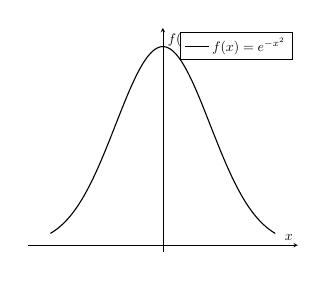
\begin{tikzpicture}[scale=0.5]
            \begin{axis}[
                axis lines=middle, % Place les axes au centre
                xlabel={$x$}, % Étiquette pour l'axe x
                ylabel={$f(x)$}, % Étiquette pour l'axe y
                domain=-30:30, % Intervalle de définition de la fonction
                samples=200, % Nombre de points pour tracer la courbe
                %grid=both, % Affiche la grille
                major grid style={line width=0.8pt,draw=gray!50}, % Style de la grille principale
                minor grid style={line width=0.4pt,draw=gray!20}, % Style de la grille secondaire
                enlargelimits=true, % Laisse un espace autour des données
                xtick=\empty, % Supprime les valeurs de l'axe x
                ytick=\empty, % Supprime les valeurs de l'axe y
                ]
                % Trace de la gaussienne
                \addplot[black, thick] {exp(-x^2*pi*0.001)};
                % Légende
                \addlegendentry{$f(x) = e^{-x^2}$}
            \end{axis}
        \end{tikzpicture}
    \end{multicols}

    Et en appliquant la transformée de Fourier, on obtient :

    \begin{multicols}{2}
        \[ \hat{\gamma}_a = a^{-1/2} \gamma_{\frac{1}{a}} \] 
        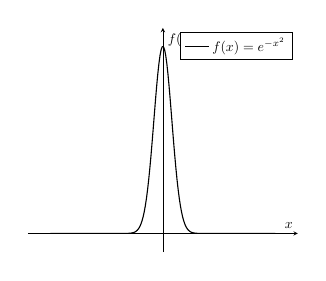
\begin{tikzpicture}[scale=0.5]
            \begin{axis}[
                axis lines=middle, % Place les axes au centre
                xlabel={$x$}, % Étiquette pour l'axe x
                ylabel={$f(x)$}, % Étiquette pour l'axe y
                domain=-5:5, % Intervalle de définition de la fonction
                samples=200, % Nombre de points pour tracer la courbe
                %grid=both, % Affiche la grille
                major grid style={line width=0.8pt,draw=gray!50}, % Style de la grille principale
                minor grid style={line width=0.4pt,draw=gray!20}, % Style de la grille secondaire
                enlargelimits=true, % Laisse un espace autour des données
                xtick=\empty, % Supprime les valeurs de l'axe x
                ytick=\empty, % Supprime les valeurs de l'axe y
                ]
                % Trace de la gaussienne
                \addplot[black, thick] {exp(-x^2*pi)};
                % Légende
                \addlegendentry{$f(x) = e^{-x^2}$}
            \end{axis}
        \end{tikzpicture}
    \end{multicols}
    
    Visuellement,la transformée de Fourier permet donc "d'isoler" les signaux d'une courbe. 
\end{example}